\chapter{Voltage Divider} \labchap{voltage_divider}
The most basic way to measure resistance is with a voltage divider.
A voltage divider consists of two resistors in series that go between an input voltage and ground, as shown in the schematic below.
The resistive sensor is placed at the $R_2$ position and we want to read the potential between the top of $R_2$ and ground, $V_{out}$ to determine the sensor's resistance.
This voltage can be determined by the equation:

\begin{equation} \labeq{voltage_divider}
    V_{out} = V_{in} \frac{R_2}{R_1 + R_2}
\end{equation}

\begin{figure}[h!]
    \caption{A typical voltage divider circuit}
    \labfig{voltage_divider}
    \centering
    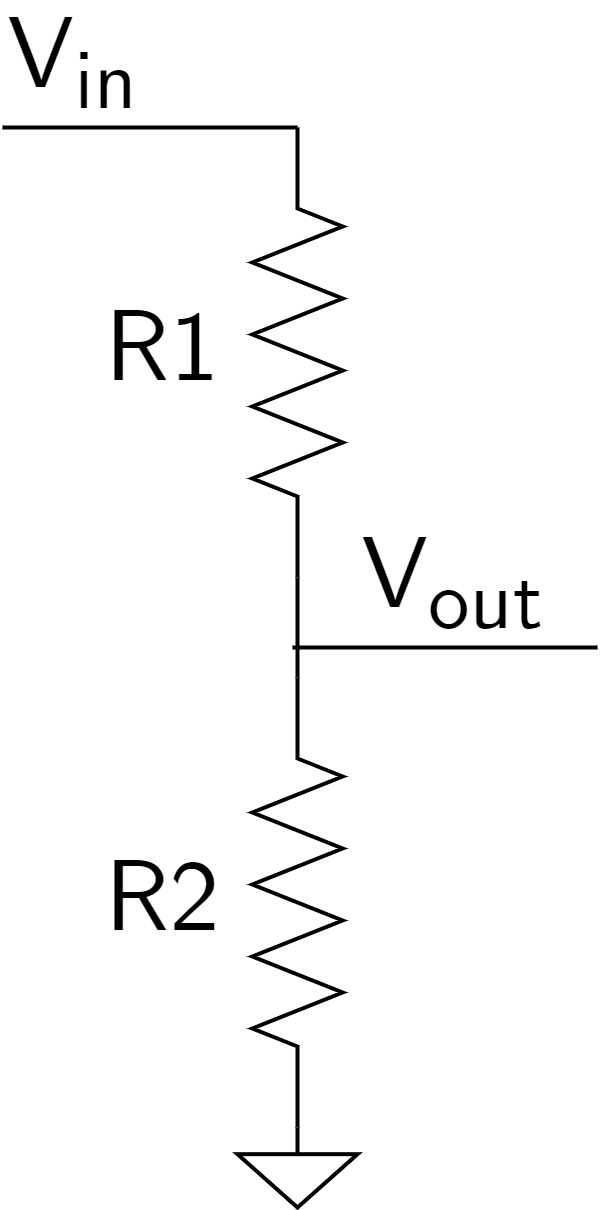
\includegraphics[height=2.5in]{appendices/voltage_divider/voltage_divider.png}
\end{figure}

\section{Example: Battery Monitor}
    Let's say the device you are bringing with you onto the roller coaster uses a 3.3V-logic microcontroller.
    It can only accept signals up to 3.3V before risking damage to its circuits.
    If you want your device to be portable, you can use a lithium polymer (LiPo) battery, but these must be carefully monitored to prevent over discharge.
    A single-cell LiPo battery has a peak voltage of 4.2V which is higher than what the microcontroller can handle.
    So, we must step down the voltage such that the peak battery voltage matches the peak input voltage of the microcontroller. \\
    
    This is a perfect application for a voltage divider, but we must first determine what two resistors will be used.
    To linearize (simplify) the problem, we will arbitrarily set $R_2 = 10\text{k} \Omega$.
    Then, we can rearrange the problem to solve for $R_1$
    
    \begin{align*}
        V_{out}                 &= V_{in} \frac{R_2}{R_1 + R_2} \\
        \frac{R_2}{R_1 + R_2}   &= \frac{V_{out}}{V_{in}} \\
        R_1 + R_2               &= \frac{V_{in} \cdot R_2}{V_{out}}\\
        R_1                     &= \frac{V_{in} \cdot R_2}{V_{out}} - R_2 \\
                                &= \frac{4.2 \cdot 10\times10^3}{3.3} - 10\times10^3 \\
                                &= 2727 \Omega
    \end{align*}

    To get a resistor that is exactly 2727 $\Omega$ is very difficult, but we can approximate this value using the much more common 2.7 k$\Omega$ resistor without introducing much error into our measurements.

    \begin{figure}[h!]
        \caption{A simple battery monitor circuit for 3.3V logic level microcontrollers.}
        \labfig{battery_monitor}
        \centering
        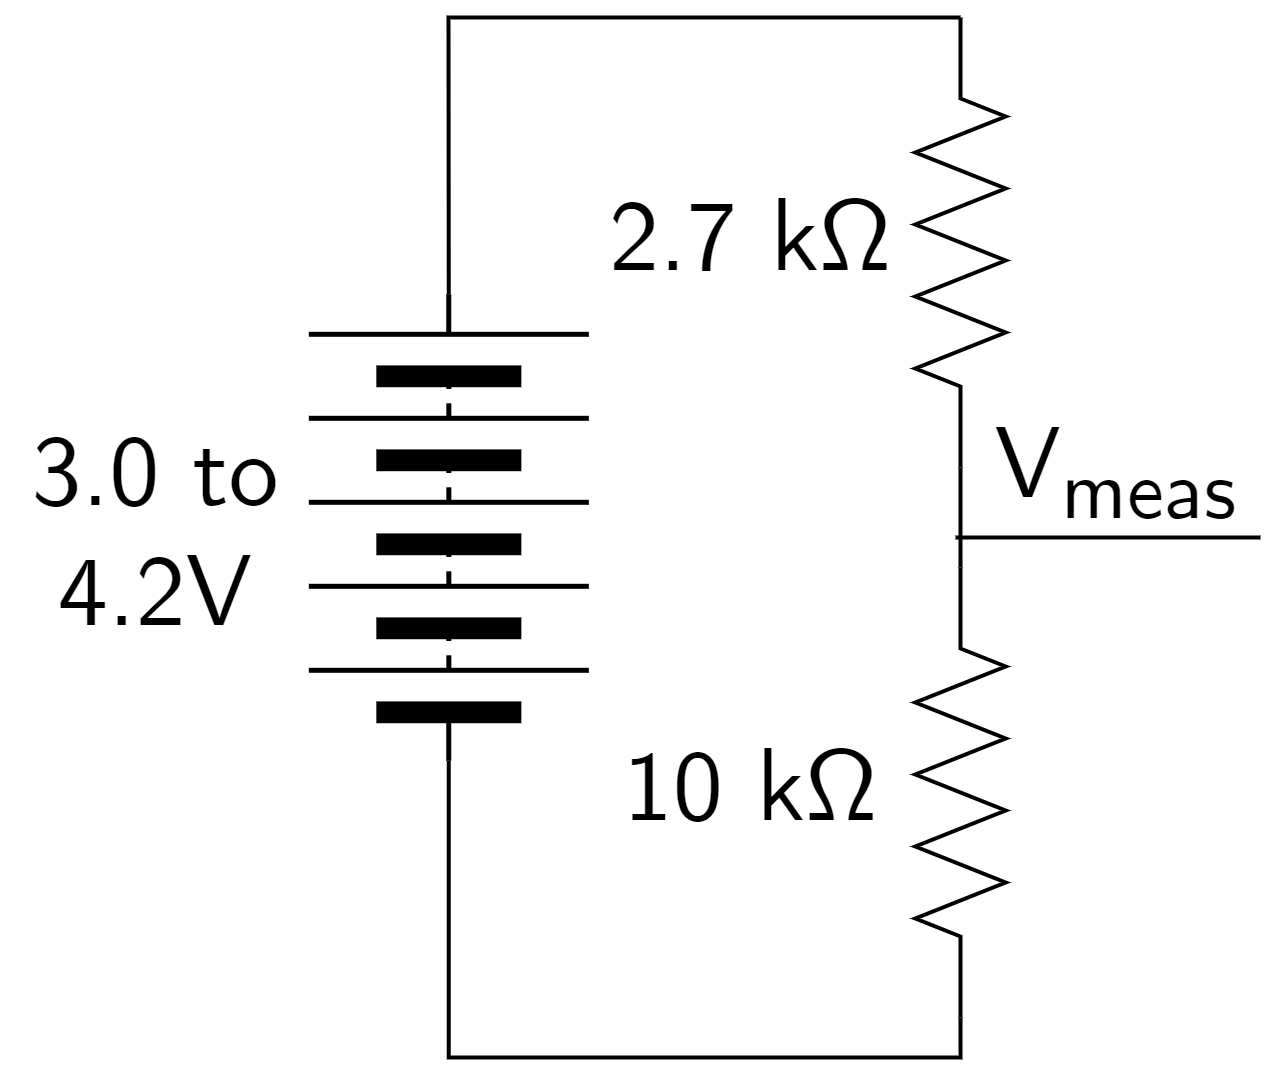
\includegraphics[height=2.5in]{appendices/voltage_divider/battery_monitor.png}
    \end{figure}